\documentclass[11pt]{article}

\usepackage[margin=1in]{geometry}
\usepackage{amsmath,amssymb,amsthm}
\usepackage{physics}
\usepackage{siunitx}
\usepackage{enumitem}
\usepackage{graphicx}
\usepackage{hyperref}

\title{The Solar System HW5}
\author{Evan Shipley-Friedt}
\date{April 21, 2026}

\begin{document}
\maketitle

\section*{Problem 1}
Textbook 10-4. Methane (CH$_4$) in Titan's atmosphere is photolyzed by solar Lyman-$\alpha$
radiation at $\SI{121.6}{nm}$:
\[
\mathrm{CH_4}+h\nu\to \mathrm{CH_3}+\mathrm{H},
\qquad
\mathrm{CH_3}+\mathrm{CH_3}\to \mathrm{C_2H_6},
\qquad
\mathrm{H}+\mathrm{H}\to \mathrm{H_2}.
\]
\begin{enumerate}[label=(\alph*)]
\item Taking the solar Lyman-$\alpha$ flux at Earth to be
$\SI{1e16}{photons\,m^{-2}\,s^{-1}}$, find the flux at Titan's orbit, $a=\SI{9.5}{AU}$,
and the flux averaged over Titan's whole surface.
\item If two photons are required to make one C$_2$H$_6$ molecule, find the C$_2$H$_6$
production rate and the CH$_4$ destruction rate per unit area.
\item Titan has surface pressure $P=\SI{1.5}{bar}$, mean molecular weight $28$, and a methane
mixing ratio of 5 percent. How long would it take to destroy all of Titan's methane? Which
assumption must be failing?
\end{enumerate}

\subsection*{Solution}
\textbf{(a) Flux}

Using inverse-square dilution,
\[
\Phi_T=\Phi_\oplus\left(\frac{1}{9.5}\right)^2
=\frac{1.0\times 10^{16}}{9.5^2}
=\SI{1.1e14}{photons\,m^{-2}\,s^{-1}}.
\]
Titan intercepts sunlight over its cross-sectional area $\pi R_T^2$, but the average flux over
the whole surface divides that light over the full area $4\pi R_T^2$:
\[
\langle \Phi_T\rangle=\Phi_T\frac{\pi R_T^2}{4\pi R_T^2}
=\frac{\Phi_T}{4}
=\boxed{\SI{2.8e13}{photons\,m^{-2}\,s^{-1}}}.
\]

\textbf{(b) Production and destruction rates}

Two CH$_4$ photolysis events give two CH$_3$ radicals, which make one C$_2$H$_6$:
\[
\dot N_{\mathrm{C_2H_6}}=\frac{\langle \Phi_T\rangle}{2}
=\boxed{\SI{1.4e13}{molecules\,m^{-2}\,s^{-1}}}.
\]
Each absorbed photon destroys one CH$_4$ molecule:
\[
\dot N_{\mathrm{CH_4}}=\langle \Phi_T\rangle
=\boxed{\SI{2.8e13}{molecules\,m^{-2}\,s^{-1}}}.
\]

\textbf{(c) Methane lifetime}

Using $P=\Sigma g_T$ with $g_T\simeq\SI{1.35}{m\,s^{-2}}$,
\[
\Sigma=\frac{P}{g_T}
=\frac{1.5\times 10^5}{1.35}
=\SI{1.1e5}{kg\,m^{-2}}.
\]
For mean molecular mass $\bar m=\SI{28e-3}{kg\,mol^{-1}}$,
\[
N_{\mathrm{tot}}=\frac{\Sigma N_A}{\bar m}
=\frac{(1.1\times 10^5)(6.022\times 10^{23})}{2.8\times 10^{-2}}
=\SI{2.4e30}{molecules\,m^{-2}}.
\]
Taking 5 percent methane,
\[
N_{\mathrm{CH_4}}=0.05N_{\mathrm{tot}}
=\SI{1.2e29}{molecules\,m^{-2}}.
\]
Thus
\[
\tau_{\mathrm{CH_4}}
=\frac{N_{\mathrm{CH_4}}}{\dot N_{\mathrm{CH_4}}}
=\frac{1.2\times 10^{29}}{2.8\times 10^{13}}
=\SI{4.3e15}{s}
=\boxed{\SI{1.4e8}{yr}}.
\]

Dimensional check:
\[
[\tau]=
\frac{\mathrm{molecules\,m^{-2}}}
{\mathrm{photons\,m^{-2}\,s^{-1}}}
\frac{\mathrm{photon}}{\mathrm{molecule}}
=\si{s}\quad \checkmark
\]
Sanity check:
\[
\frac{4.5\times 10^9\ \mathrm{yr}}{1.4\times 10^8\ \mathrm{yr}}\approx 33.
\]
So Titan's methane should have been destroyed many times over. The closed-inventory assumption
is failing: atmospheric methane must be resupplied from surface or interior reservoirs. Shielding
by upper-atmosphere photochemical products also means the full methane column is not simply
removed at the incident Lyman-$\alpha$ rate.

\newpage
\section*{Problem 2}
Textbook 11-10. The isotope $^{187}$Re decays to $^{187}$Os with half-life
$t_{1/2}=\SI{4.16e10}{yr}$. The measured isotope ratios are:
\[
\begin{array}{c|cccccccc}
{}^{187}\mathrm{Re}/{}^{188}\mathrm{Os}
&0.664&0.669&0.604&0.484&0.512&0.537&0.414&0.369\\
\hline
{}^{187}\mathrm{Os}/{}^{188}\mathrm{Os}
&0.148&0.148&0.143&0.133&0.136&0.138&0.128&0.124
\end{array}
\]
\begin{enumerate}[label=(\alph*)]
\item Plot $^{187}\mathrm{Os}/{}^{188}\mathrm{Os}$ against
$^{187}\mathrm{Re}/{}^{188}\mathrm{Os}$.
\item Fit a straight line and use its slope to find the rock age.
\item Plot theoretical isochrones through the same initial
$^{187}\mathrm{Os}/{}^{188}\mathrm{Os}$ ratio and read off the age.
\end{enumerate}

\subsection*{Solution}
The isochron equation is
\[
\frac{{}^{187}\mathrm{Os}}{{}^{188}\mathrm{Os}}
=
\left(\frac{{}^{187}\mathrm{Os}}{{}^{188}\mathrm{Os}}\right)_0
+\left(e^{t/\tau}-1\right)
\frac{{}^{187}\mathrm{Re}}{{}^{188}\mathrm{Os}},
\qquad
\tau=\frac{t_{1/2}}{\ln 2}.
\]
The mean lifetime is
\[
\tau=\frac{4.16\times 10^{10}}{0.6931}
=\SI{6.00e10}{yr}.
\]
Fitting $y=mx+b$ gives
\[
m=0.0803,\qquad b=0.0946.
\]
Solving for the age,
\[
m=e^{t/\tau}-1
\]
\[
t=\tau\ln(1+m)
=(6.00\times 10^{10})\ln(1.0803)
=\SI{4.63e9}{yr}.
\]
Therefore
\[
\boxed{t\approx\SI{4.6}{Gyr}},
\qquad
\boxed{\left(\frac{{}^{187}\mathrm{Os}}{{}^{188}\mathrm{Os}}\right)_0\approx 0.0946}.
\]

\begin{center}
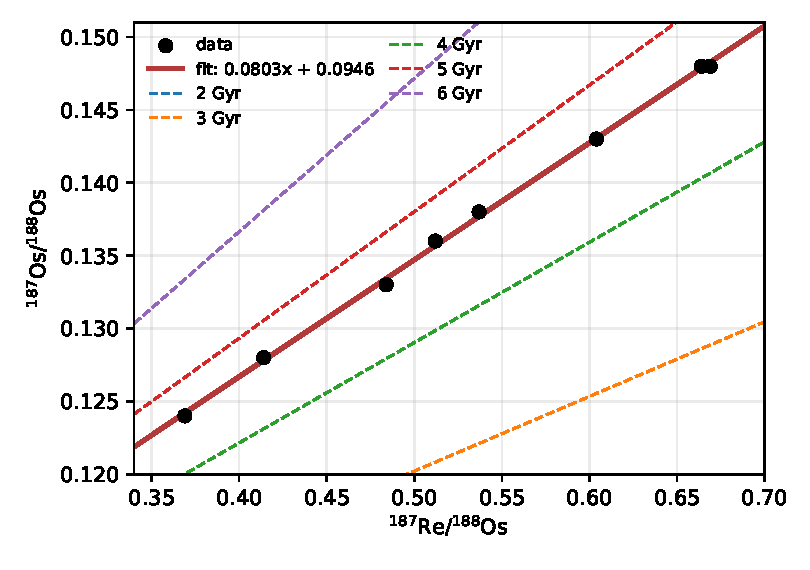
\includegraphics[width=0.78\textwidth]{re_os_isochrons.pdf}
\end{center}

For reference, the isochrone slopes are:
\[
\begin{array}{c|ccccc}
t\ (\mathrm{Gyr})&2&3&4&5&6\\
\hline
e^{t/\tau}-1&0.0339&0.0513&0.0690&0.0869&0.105
\end{array}
\]
The fitted slope lies between the 4 Gyr and 5 Gyr isochrones, closer to 5 Gyr.

For small slopes, $e^{t/\tau}-1\simeq t/\tau$, so
$t\simeq m\tau\simeq (0.080)(6.00\times 10^{10})=\SI{4.8e9}{yr}$, close to the exact
logarithmic result.

\newpage
\section*{Problem 3}
An exam question that nobody got completely correct:

Consider a spherically symmetric planet with radius $R$, density $\rho(r)$, and angular velocity
$\omega(r)$ that may vary with radius. Derive shell and integral expressions for:
\begin{enumerate}[label=(\alph*)]
\item mass $dM$ and $M(R)$,
\item moment of inertia $dI$ and $I(R)$,
\item rotational kinetic energy $dT$ and $T(R)$,
\item angular momentum $dL$ and $L(R)$,
\item gravitational binding energy $dU$ and $U(R)$.
\end{enumerate}
Useful facts:
\[
\begin{aligned}
dM&=4\pi r^2\rho(r)\,dr,&
dI&=\frac{2}{3}r^2\,dM,\\
dT&=\frac{1}{2}\omega^2(r)\,dI,&
dL&=\omega(r)\,dI.
\end{aligned}
\]

\subsection*{Solution}
\textbf{(a) Mass}

Using spherical shells,
\[
\boxed{dM=4\pi r^2\rho(r)\,dr}
\]
and integrating from 0 to $R$,
\[
\boxed{M(R)=\int_0^R 4\pi r^2\rho(r)\,dr}.
\]
Check: for $\rho(r)=\rho_0$,
\[
M(R)=4\pi\rho_0\int_0^R r^2\,dr
=\frac{4}{3}\pi R^3\rho_0\quad \checkmark.
\]
Units:
\[
[r^2\rho\,dr]=\si{m^2}\,\si{kg\,m^{-3}}\,\si{m}=\si{kg}\quad \checkmark.
\]

\textbf{(b) Moment of inertia}

Substituting $dM$ into the thin-shell moment of inertia,
\[
\boxed{dI=\frac{2}{3}r^2\,dM
=\frac{8\pi}{3}r^4\rho(r)\,dr}
\]
so
\[
\boxed{I(R)=\frac{8\pi}{3}\int_0^R r^4\rho(r)\,dr}.
\]
Check: for $\rho(r)=\rho_0$,
\[
I=\frac{8\pi}{3}\rho_0\int_0^R r^4\,dr
=\frac{8\pi}{15}\rho_0R^5.
\]
Using $M=(4/3)\pi R^3\rho_0$,
\[
I=\frac{2}{5}MR^2\quad \checkmark.
\]
If all the mass is concentrated at $r=0$, then $r^2dM\to0$ and $I\to0\quad \checkmark$.

\textbf{(c) Rotational kinetic energy}

Using $dT=(1/2)\omega^2(r)dI$,
\[
\boxed{dT=\frac{4\pi}{3}r^4\rho(r)\omega^2(r)\,dr}
\]
and
\[
\boxed{T(R)=\frac{4\pi}{3}\int_0^R r^4\rho(r)\omega^2(r)\,dr}.
\]
Check: for rigid rotation, $\omega(r)=\omega_0$,
\[
T=\frac{1}{2}\omega_0^2
\left(\frac{8\pi}{3}\int_0^R r^4\rho(r)\,dr\right)
=\frac{1}{2}I\omega_0^2\quad \checkmark.
\]
If $\omega\to0$, then $T\to0\quad \checkmark$.

\textbf{(d) Angular momentum}

Using $dL=\omega(r)dI$,
\[
\boxed{dL=\frac{8\pi}{3}r^4\rho(r)\omega(r)\,dr}
\]
and
\[
\boxed{L(R)=\frac{8\pi}{3}\int_0^R r^4\rho(r)\omega(r)\,dr}.
\]
Check: for rigid rotation, $\omega(r)=\omega_0$,
\[
L=\omega_0
\left(\frac{8\pi}{3}\int_0^R r^4\rho(r)\,dr\right)
=I\omega_0\quad \checkmark.
\]
If $\omega\to0$, then $L\to0\quad \checkmark$.

\textbf{(e) Gravitational binding energy}

Building the planet shell-by-shell, bringing a shell $dM$ from infinity to radius $r$ gives
\[
\boxed{dU=-\frac{GM(r)\,dM}{r}}.
\]
This counts each pair once, so there is no extra factor of $1/2$. Substituting $dM$,
\[
\boxed{dU=-4\pi G\,r\,\rho(r)M(r)\,dr}
\]
where
\[
M(r)=\int_0^r 4\pi r'^2\rho(r')\,dr'.
\]
Therefore
\[
\boxed{U(R)=-4\pi G\int_0^R r\,\rho(r)M(r)\,dr}.
\]
The enclosed mass is $M(r)$, not the final total mass $M(R)$.

Check: for $\rho(r)=\rho_0$,
\[
M(r)=\frac{4}{3}\pi r^3\rho_0
\]
so
\[
U=-4\pi G\rho_0\int_0^R r\left(\frac{4}{3}\pi r^3\rho_0\right)\,dr
=-\frac{16\pi^2G\rho_0^2}{3}\frac{R^5}{5}
=-\frac{16\pi^2G\rho_0^2R^5}{15}.
\]
Substituting $\rho_0=3M/(4\pi R^3)$,
\[
U=-\frac{16\pi^2G}{15}\frac{9M^2}{16\pi^2R}
=-\frac{3}{5}\frac{GM^2}{R}\quad \checkmark.
\]
The sign is negative for a bound object, and the units are
\[
\frac{\si{m^3}}{\si{kg\,s^2}}\,
\si{m}\,
\frac{\si{kg}}{\si{m^3}}\,
\si{kg}\,
\si{m}
=\si{kg\,m^2\,s^{-2}}=\si{J}\quad \checkmark.
\]

\end{document}
